\section{Game Design}\label{section:game-design}
The intended design of the game will be similar to \textit{Squash}, while retaining the graphics of \textit{Pong}. 
In \figref{figure:game-layout} the layout of the game board can be seen. 
The basic elements of the game are the ball, the paddle, the walls, and power-ups. 
The main objective of the game is to prevent the ball from moving past the paddle.

\begin{figure}[h]
	\centering
	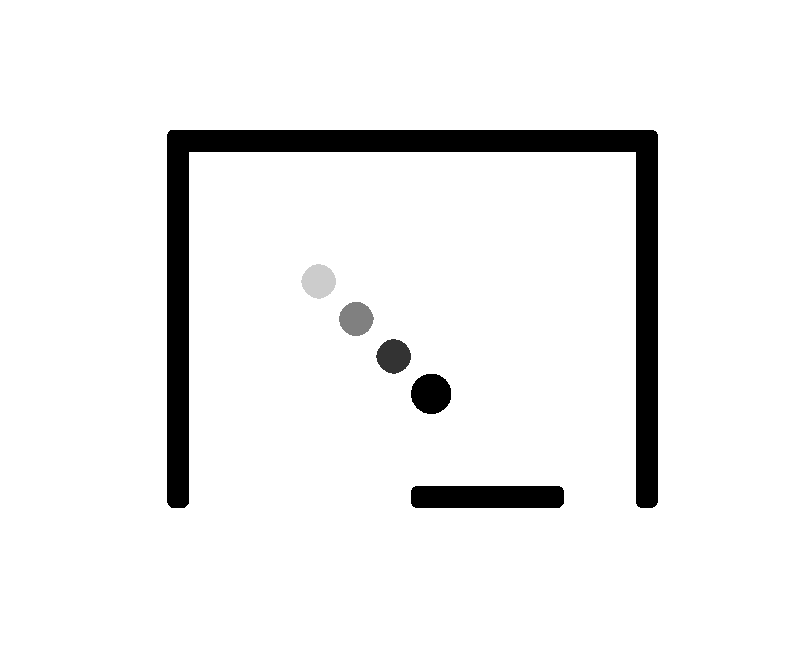
\includegraphics[scale = 0.3]{media/design/game-layout.pdf}
	\caption{The layout of the game board}
	\label{figure:game-layout}
\end{figure}

An important game design aspect is the control of the paddle, which in this project relies on dead reckoning for movement tracking. 
It means if the player moves left or right, the paddle will follow his movements. 

While the basic elements of the game are simple, some additional features have been added to the game to enhance the user experience.
Some of these features include a scoring system and power-ups.
The score is based on the time the player keeps the game alive, meaning as long as there is at least one ball on the board, the score increases.
Power-ups could increase the size of the paddle, get an extra ball on the board, or slow the speed of the balls, and negative power-ups could decrease the paddle size, increase the speed of the balls, or decrease the score.
A story board of how the game should work can be seen in \figref{figure:story-board}.
\begin{figure}[H]
	\centering
	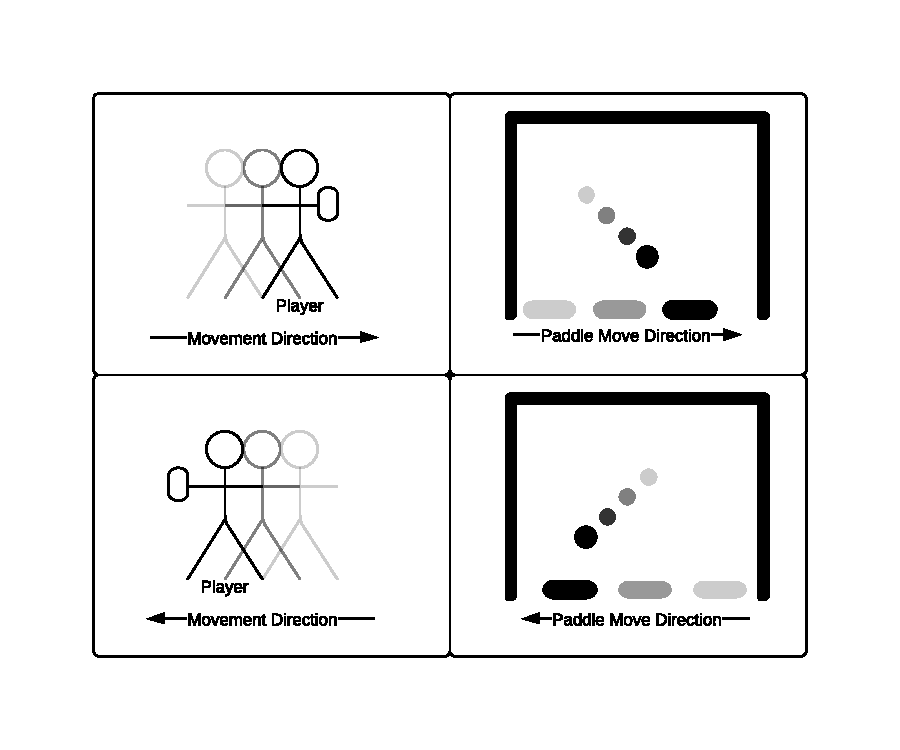
\includegraphics[trim = 0cm 1.5cm 0cm 1.5cm, clip, scale = 0.75]{media/design/story-board.pdf}
	\caption{A storyboard of how the game is played}
	\label{figure:story-board}
\end{figure}

%FEATURES
%POWERUP: BIGGER PADDLE, MOAR BAALS, SLOW ALL BALLS, DOUBLE POINTS FOR x TIME, 
%NEGATIVE POWERUPS: SMALLER PADDLE, FASTER BAAALS, FLASHING BALLS, -x\% score, inverted controls
%HIGHSCORE

